\documentclass[conf]{new-aiaa}
%\documentclass[journal]{new-aiaa} for journal papers
\usepackage[utf8]{inputenc}

\usepackage{graphicx}
\usepackage{amsmath}
\usepackage[version=4]{mhchem}
\usepackage{siunitx}
\usepackage{longtable,tabularx}
\setlength\LTleft{0pt} 

\title{Modifying Operational Fleet Paths to Better Track Moving Objects}

\author{Leonardo Pi{\~{n}}ero-P{\'{e}}rez\footnote{Engineer I, Control Laws, 4813 Bob Wills Dr., AIAA Member.}}
\affil{Bell Flight, Arlington, TX, 76019}

\begin{document}

\maketitle

\begin{abstract}
Insert Abstract Here. It should be one paragraph long (not an introduction) and complete in itself (no reference numbers). It should indicate subjects dealt with in the paper and state the objectives of the investigation. Newly observed facts and conclusions of the experiment or argument discussed in the paper must be stated in summary form; readers should not have to read the paper to understand the abstract. The abstract should be bold, indented 3 picas (1/2'') on each side, and separated from the rest of the document by blank lines above and below the abstract text..
\end{abstract}

\section{Nomenclature}

{\renewcommand\arraystretch{1.0}
\noindent\begin{longtable*}{@{}l @{\quad=\quad} l@{}}
$A$  & amplitude of oscillation \\
$a$ &    cylinder diameter \\
$C_p$& pressure coefficient \\
$Cx$ & force coefficient in the \textit{x} direction \\
$Cy$ & force coefficient in the \textit{y} direction \\
c   & chord \\
d$t$ & time step \\
$Fx$ & $X$ component of the resultant pressure force acting on the vehicle \\
$Fy$ & $Y$ component of the resultant pressure force acting on the vehicle \\
$f, g$   & generic functions \\
$h$  & height \\
$i$  & time index during navigation \\
$j$  & waypoint index \\
$K$  & trailing-edge (TE) nondimensional angular deflection rate
\end{longtable*}}

% ====================================================================
% INTRODUCTION
% ---------------------
% ====================================================================
\section{Introduction}
\lettrine{T}{his} work establishes a methodology for tracking moving objects with an existing fleet of aircraft. An ``object'' is defined as any detectable information moving spatially as a \emph{cyclical} function of time, such as automobile traffic for a given weekday, other aircraft for their given schedules, or air pollution for a given a week. In real-world applications of this methodology, a fleet of unmanned aerial vehicles is the intended platform for the following reasons:
\begin{enumerate}
\item Operational flexibility
\item Tendency to operate in dense urban environments
\item Low and slow cruise conditions
\item Potential high density per square-mile
\end{enumerate}

Regardless, the algorithm is agnostic to whatever vehicle platform is used so long as its path can be freely changed. However, to meet this criteria, this will almost certainly be an aerial platform (though special use cases could also include submersibles or maneuverable spacecraft). This methodology would likely be inadequate to implement on ground fleets which have to cope with the unknown guidance variables accompanied by navigating through non-flat terrain.

The platform's minimum and maximum velocity is defined to place limits on how a path can be altered as a function of time. Additionally, a constant ``sight'' parameter is used to establish the spatial range of sight for the platform aircraft. In reality, this sight parameter is not constant throughout the flight, since low-altitude flight profiles are sensitive to large ground features such as terrain or tall buildings obstructing the full view. It is also important to note that if the altitude is non-constant, the cone of sight increases with the increased squared altitude.\cite{zorbas2013energyefficientmobiletracking}
% INSERT REFERENCE FOR CHANGING UAV ALTITUDE HERE





% ====================================================================
% BACKGROUND
% ---------------------
% ====================================================================

\section{Background}

Related Work, state-of-the-art.


% ====================================================================
% PROBLEM STATEMENT
% ---------------------
% ====================================================================

\section{Problem Statement}

As discussed in the introduction, a fleet of unmanned aerial vehicles provides the best platform in real-world applications of this methodology. This fleet will have consistent locations at which the aerial vehicles will be scheduled to arrive at and depart from at specified times. Given this schedule, the goal is to not disturb the existing paths such that the side benefit of using the fleet for survey operations does not interfere with the main mission of this fleet, whatever it may be. This section will propose some potential side-benefits and applications of the proposed methodology.

% Google Maps Validation
% ---------------------
\subsection{Google Maps Validation}
The Google Maps application has a solution to the problem of tracking automobile traffic. The application aggregates the real-time location data generated by drivers using Google Maps or Android phones while having location services enabled \cite{barth2009googlemaps}. The methodology proposed in this paper can be used to assess and validate the accuracy of this existing system. The validated data could also be used to determine the number of users actually broadcasting their anonymous location data via Google Maps or Android.

% Atmospheric Survey
% ---------------------
\subsection{Atmospheric Survey}
While the previous use case is used to validate existing data, vehicles may be used to generate novel data for non-visual objects, such as air pollution. Fleet vehicles may be equipped with instrumentation designed to detect the presence of particulates. The ``sight'' parameter could be the expected size of a particulate cloud or the region of airspace for which detection will represent a cloud's presence. For this use case, the parameter has a slight change in definition from that stated in the introduction. This is due to the fact that particulate detection would occur at the exact location of the aerial vehicle, rather than at a distance via ranged vision.

% Migration Patterns
% ---------------------
\subsection{Migration Patterns}

Another potential use case for this 



% ====================================================================
% METHODOLOGY
% ---------------------
% ====================================================================

\section{Methodology}

The following section outlines the methodology used to determine the path alterations. The algorithm and its user interface is run on a Flask server, which extracts and stores simulation data via connection to a MySQL database hosted on the local machine. The source code can be found at \url{https://github.com/Leonardo767/aiaa2019-publication}, where everything except static cascading styling sheets (for aesthetics) is original work of the author. Inside the source code sample, there are two main sections: ``lib'' and ``src'', which hold the code for application utilities and the algorithm, respectively.

% Application Architecture
% ---------------------
\subsection{Application Architecture}
The application is run on a Flask server on the local machine. This was built to accelerate the development process by providing a means for the author to assess the incremental results generated by the optimization algorithm. The application was developed in the order of the workflow shown in Fig.~\ref{app-architecture}, beginning with the geographical data. This data contains information about the geography to be surveyed, such as the boundary dimensions, references to airports contained, and the  flight manifests referenced by said referenced airports. From here, flight paths can be constructed by extracting and manipulating the stored geographical information.

The next step is to input simulated objects. At the top level, the user can select simulation suites which represent the total movement of all objects for a given geographical region. It is important to note that this data is unknown the fleet operator, and is only implemented here for the sole purpose of this \emph{simulated} data to act as an evaluation of the algorithm from an omniscient perspective. The individual objects themselves and their respective path points as a function of time can be edited within the MySQL database (structured query language database).

The settings input is used to add any additional simulation settings such as the load card used or fleet vehicle properties such as allowable velocity and range of sight. Within this page, an overall preview map is available of the region.

These data are fed into a MySQL database that the Flask app can interact with. It is from this database that the algorithm pulls information and packages its results per iteration. From these results, the plots of the altered paths are generated.

\begin{figure}[hbt!]
\centering
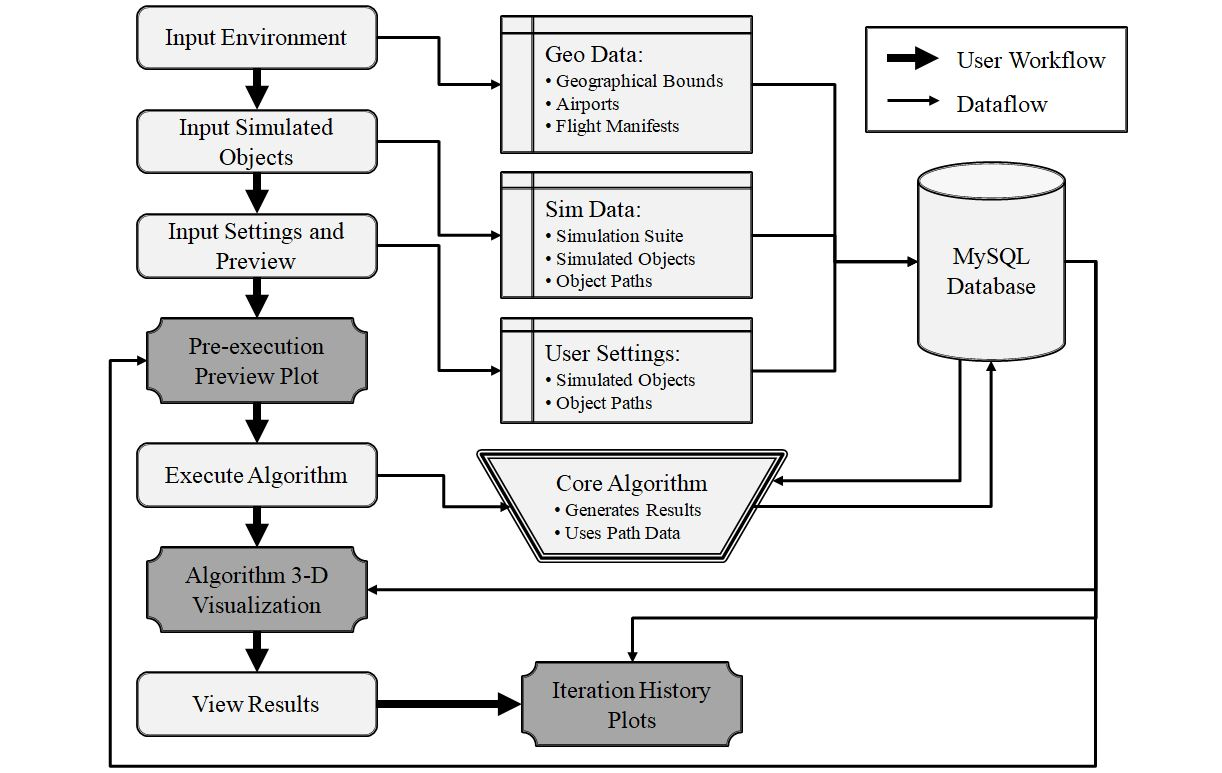
\includegraphics[width=1\textwidth]{figs/app-architecture}
\caption{Application architecture built to interface with core algorithm.}
\label{app-architecture}
\end{figure}

The application then prompts the user to an execution page, where the number of iterations and type of execution is defined by one of four selected run-modes:
\begin{enumerate}
\item \emph{Reset}: resets iteration value and does one full iteration
\item \emph{Iteration++}: runs the next iteration
\item \emph{Execute Completely}: runs for iterations defined in execution settings
\item \emph{Debug (no plot)}: outputs via machine terminal, used for development
\end{enumerate}

% Algorithm Architecture
% ---------------------
\subsection{Algorithm Architecture}
The algorithm is designed as it would operate in reality: the only information that is passed into it is the known operational flight path and the simulated contact with the target objects. The fleet will fly its initial flight paths, and the coincidental contact made with the target objects (based on the sight parameter) provide the first iteration's input. From here, the following sub-sections will explain what each component of the core algorithm in Fig.~\ref{algo-architecture} does to help compute what the next iteration of the altered path will be.

\begin{figure}[hbt!]
\centering
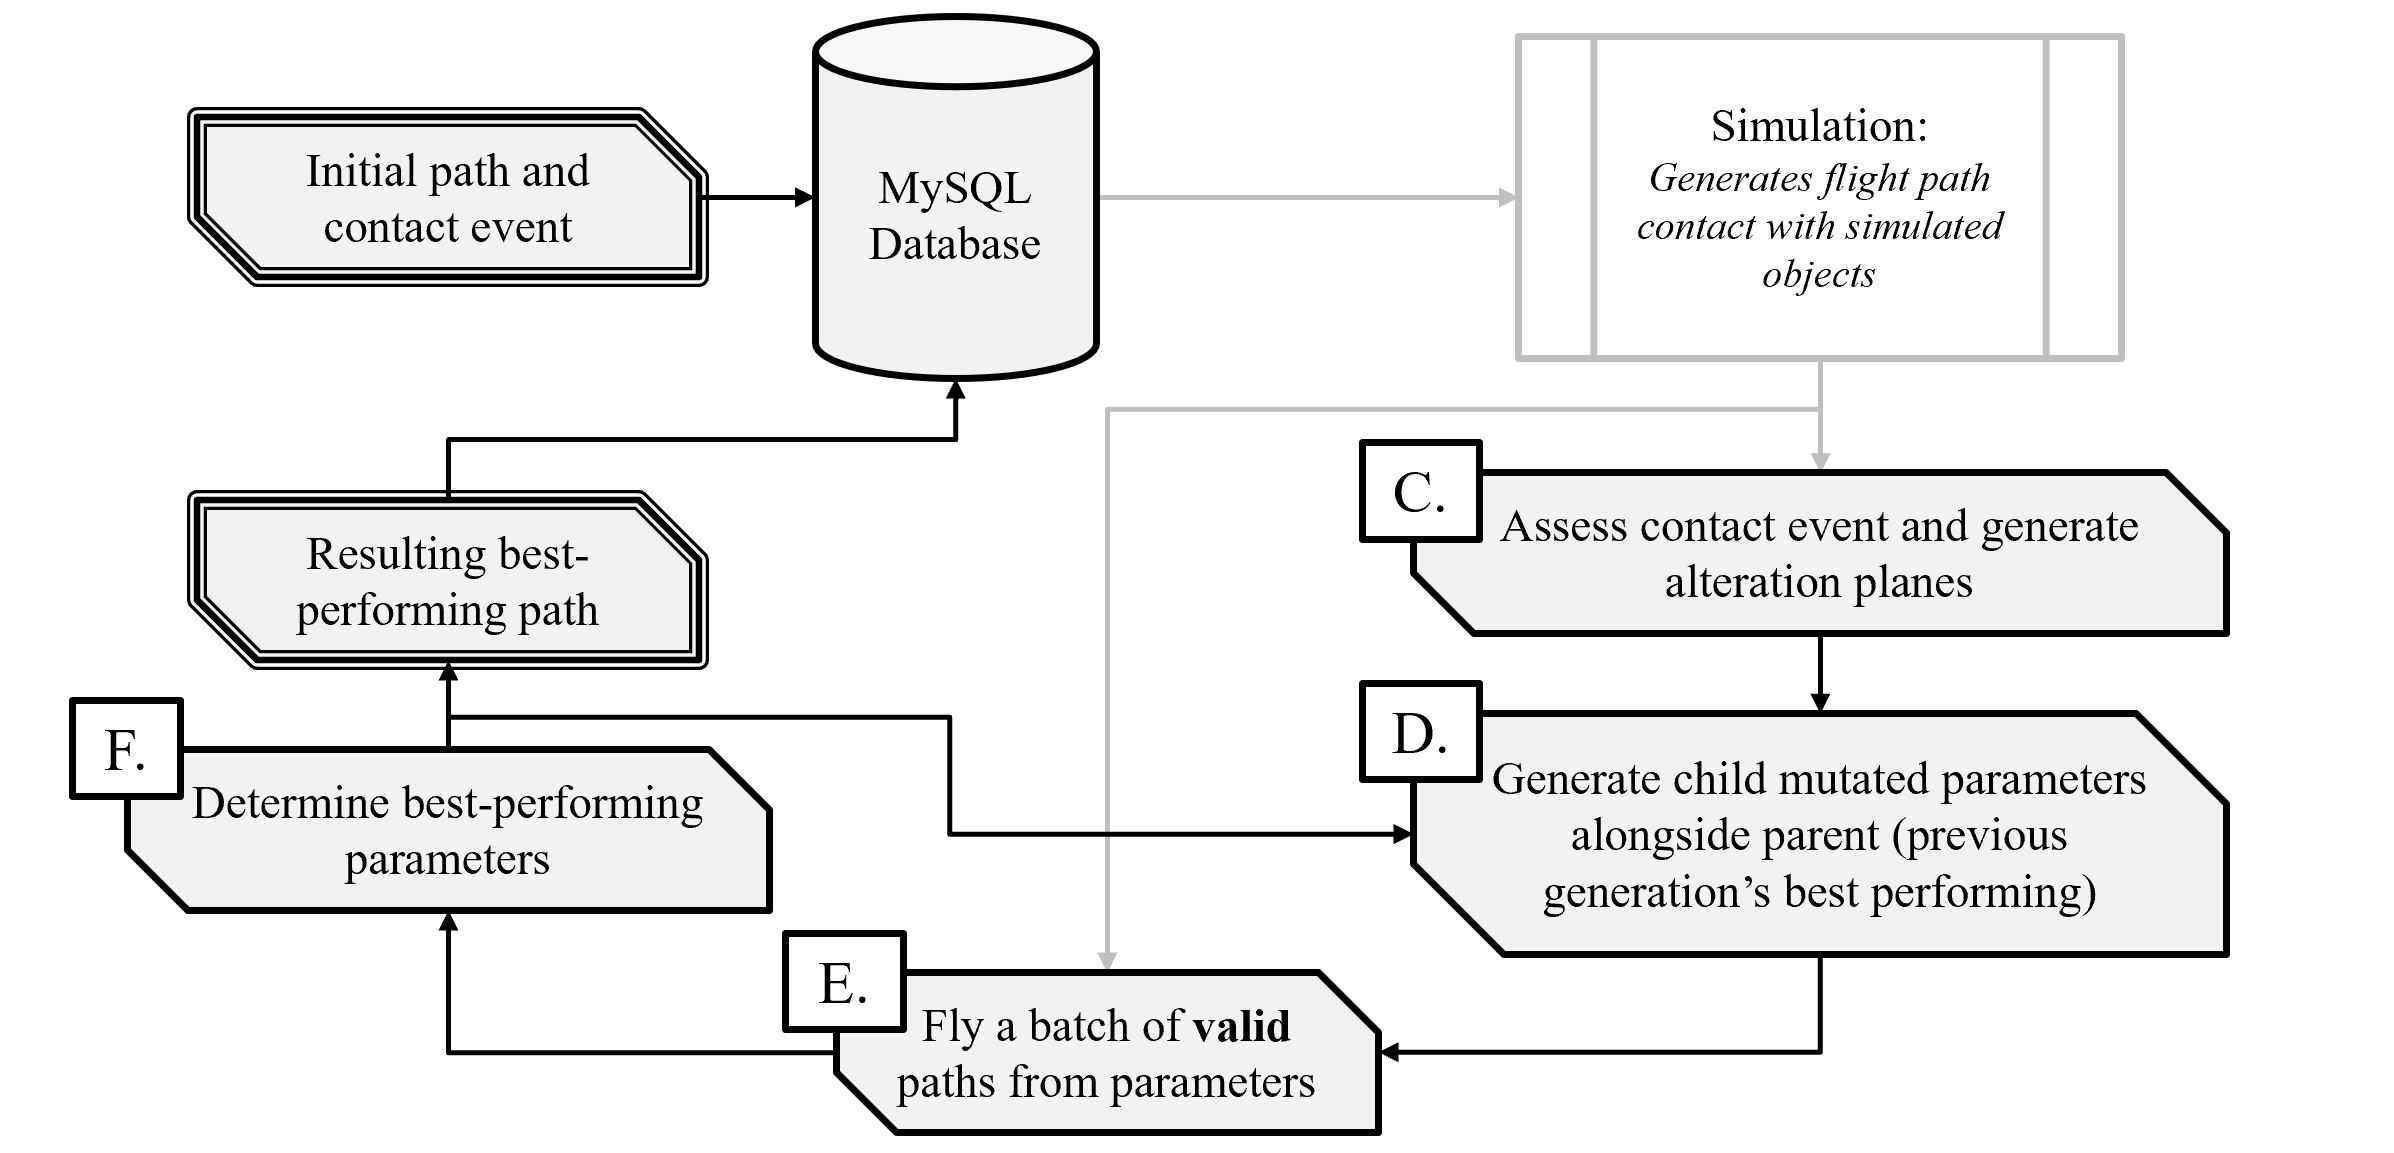
\includegraphics[width=1\textwidth]{figs/algo-architecture}
\caption{Top-level architecture of core algorithm.}
\label{algo-architecture}
\end{figure}

\subsubsection{Assessing Contact Points}
Upon receiving information about the instances of contact with the target object, the first operation is to assess some basic properties about this event. These are inputs required to inform a devised heuristic. For each flight leg, the first and last seen location of the sim object is recorded. These two points serve as anchoring points for distance vectors created between these two locations and the locations of each path node. The alteration vector for each node will be determined from the components of each node's two respective distance vectors, as shown in Fig.~\ref{heuristic-diagram}.

\begin{figure}[hbt!]
\centering
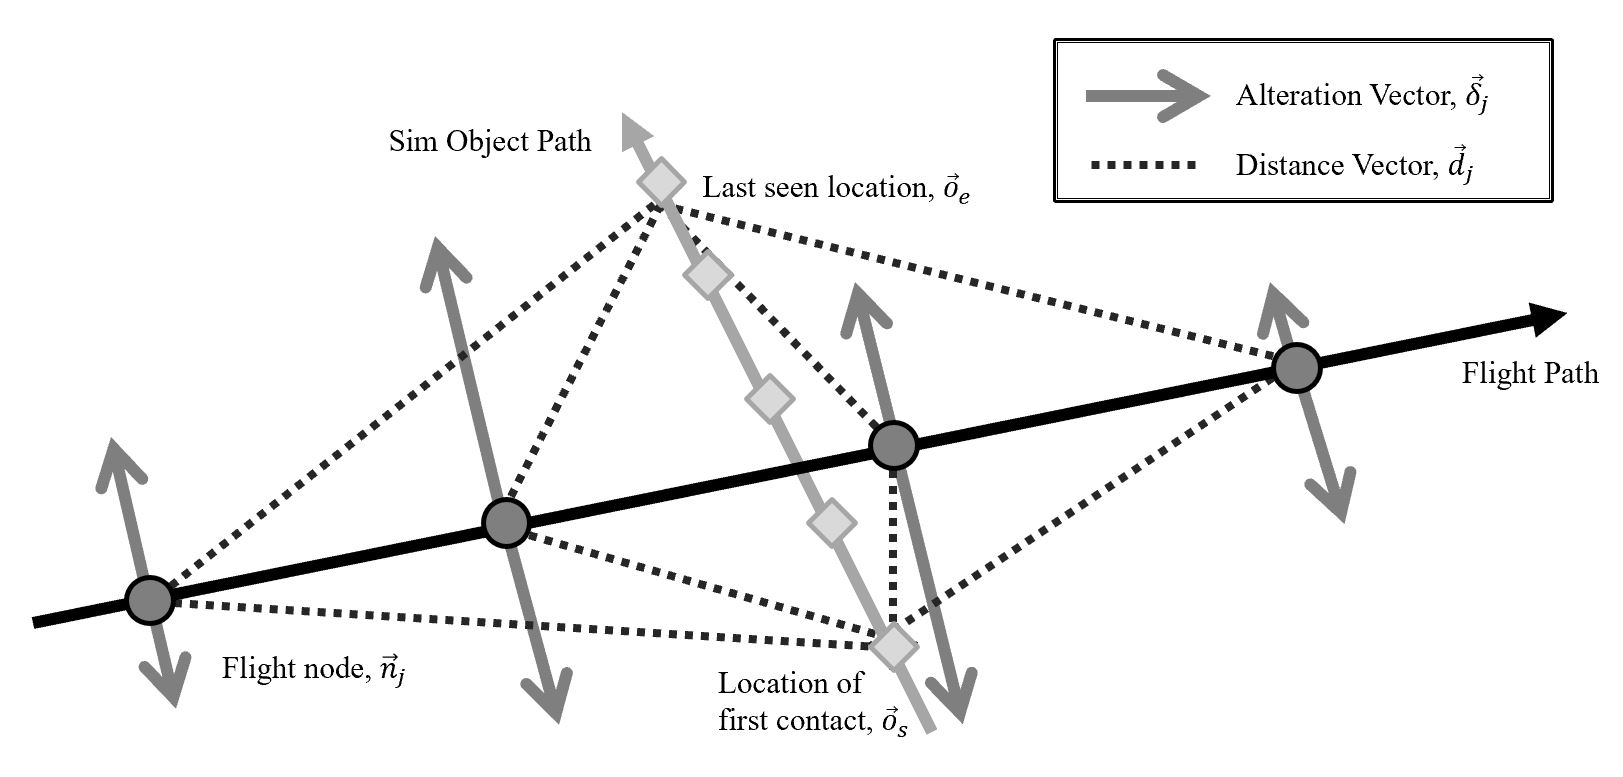
\includegraphics[width=1\textwidth]{figs/heuristic-diagram}
\caption{Visualization of heuristic for determining alteration vector per node.}
\label{heuristic-diagram}
\end{figure}

For each node, the weighted sum of the two anchored vectors will drive its new location for the next iteration of the path. Said weighting will be determined by tuned parameters. For each iteration $i$, the determination of this alteration vector is of size $n$ and is defined in Eq. (\ref{change_vector_eqn}).

\begin{equation}
\label{change_vector_eqn}
\vec{{\Delta}{n}} = {{\delta}}_i\circ{\vec{d}} = \left({{\delta}_{d_s}}\circ{{\delta}_{d_e}}\circ{{\delta}_{\theta_s}}\circ{{\delta}_{\theta_e}}\circ{{\delta}_n}\right)_i\circ{\vec{d}}
\end{equation}

Each of the Hadamard factors of $\delta$ is determined from Eqs. \ref{delta_d_se_eqn}, \ref{delta_theta_se_eqn}, and \ref{delta_n_eqn}. The parameters $d$, $\theta$, and $j$ for each node are based on the contact event with the sim object and are described in the nomenclature.

\begin{equation}
\label{delta_d_se_eqn}
\delta_{d_{\left\{s,e\right\}}} = \exp\left({-\beta_{d_{\left\{s,e\right\}}}\frac{\left\|\vec{d}\right\|^2}{2\sigma_{d_{\left\{s,e\right\}}}^2}}\right)
\end{equation}

\begin{equation}
\label{delta_theta_se_eqn}
\delta_{\theta_{\left\{s,e\right\}}} = \exp\left({-\beta_{\theta_{\left\{s,e\right\}}}\frac{{\left(\theta - \frac{\pi}{2}\right)}^2}{2\sigma_{\theta_{\left\{s,e\right\}}}^2}}\right)
\end{equation}

\begin{equation}
\label{delta_n_eqn}
\delta_n = \exp\left({-\beta_n\frac{j^2}{2\sigma_{\theta_n}^2}}\right)
\end{equation}

\subsubsection{Compute Resulting Cost}

\subsubsection{Tuned Path Alteration}


% Visualization
% ---------------------
\subsection{Visualization}
The abstract should appear at the beginning of your paper. 

\subsection{Nomenclature}
Papers with many symbols may benefit from a nomenclature list that defines all symbols with units, inserted between the abstract and the introduction. If one is used, it must contain all the symbology used in the manuscript, and the definitions should not be repeated in the text. In all cases, identify the symbols used if they are not widely recognized in the profession. Define acronyms in the text, not in the nomenclature.

\subsection{Footnotes and References}
Footnotes, where they appear, should be placed above the 1'' margin at the bottom of the page. To insert footnotes into the template, use the Insert>Footnote feature from the main menu as necessary. Numbered footnotes as formatted automatically in the template are acceptable, but superscript  symbols are the preferred AIAA style, *, $\dag$, $\ddag$, \S, \P, **, $\dag\dag$, $\ddag\ddag$, \S\S, etc.

List and number all references at the end of the paper. Corresponding bracketed numbers are used to cite references in the text \cite{vatistas1986reverse}, including citations that are an integral part of the sentence (e.g., ``It is shown in \cite{dornheim1996planetary} that\ldots '') or follow a mathematical expression: ``$A^{2} + B = C$ (Ref.~\cite{terster1997nasa}).'' For multiple citations, separate reference numbers with commas \cite{peyret2012computational,oates1997aerothermodynamics}, or use a dash to show a range \cite{volpe1994techniques,thompsonspacecraft,chi1993fluid}. Reference citations in the text should be in numerical order.

In the reference list, give all authors' names; do not use ``et al.''. Papers that have not been published should be cited as ``unpublished''; papers that have been submitted or accepted for publication should be cited as ``submitted for publication.'' Private communications and personal website should appear as footnotes rather than in the reference list.

References should be cited according to the standard publication reference style (for examples, see the ``References'' section of this template). Never edit titles in references to conform to AIAA style of spellings, abbreviations, etc. Names and locations of publishers should be listed; month and year should be included for reports and papers. For papers published in translation journals, please give the English citation first, followed by the original foreign language citation.

\subsection{Images, Figures and Tables}
All artwork, captions, figures, graphs, and tables will be reproduced exactly as submitted. Be sure to position any figures, tables, graphs, or pictures as you want them printed. AIAA will not be responsible for incorporating your figures, tables, etc. (Company logos and identification numbers are not permitted on your illustrations.)

Do not insert your tables and figures in text boxes. Figures should have no background, borders, or outlines. In the \LaTeX{} template, use the ``caption'' command to type caption text. Captions are bold with a single tab (no hyphen or other character) between the figure number and figure description.

% \begin{table}
% \caption{\label{tab:table1} Transitions selected for thermometry}
% \centering
% \begin{tabular}{lcccccc}
% \hline
% & Transition& & \multicolumn{2}{c}{}\\\cline{2-2}
% Line& $\nu''$& & $J'' $& Frequency, cm$^{-1}$& $FJ$, cm$^{-1}$& $G\nu $, cm$^{-1}$\\\hline
% a& 0& P$_{12}$& 2.5& 44069.416& 73.58& 948.66\\
% b& 1& R$_{2}$& 2.5& 42229.348& 73.41& 2824.76\\
% c& 2& R$_{21}$& 805& 40562.179& 71.37& 4672.68\\
% d& 0& R$_{2}$& 23.5& 42516.527& 1045.85& 948.76\\
% \hline
% \end{tabular}
% \end{table}


\begin{figure}[hbt!]
\centering
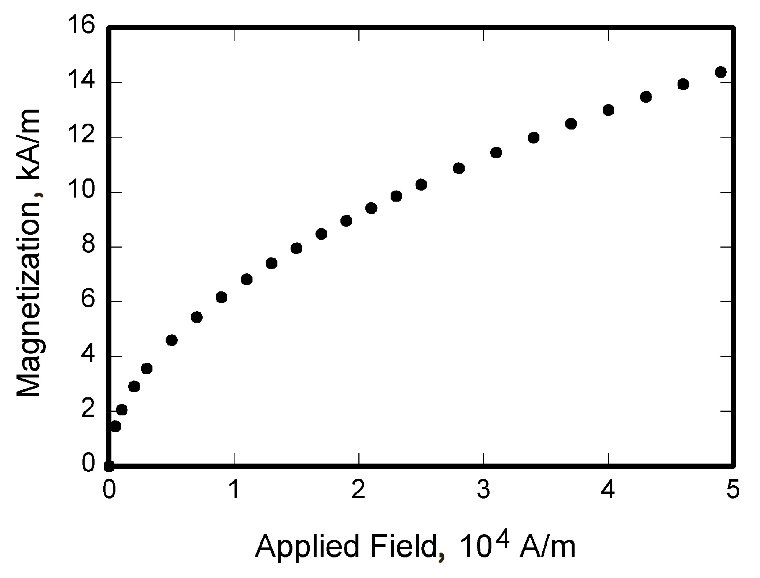
\includegraphics[width=.5\textwidth]{figs/graph}
\caption{Magnetization as a function of applied fields.}
\end{figure}

Place figure captions below all figures; place table titles above the tables. If your figure has multiple parts, include the labels ``a),'' ``b),'' etc. below and to the left of each part, above the figure caption. Please verify that the figures and tables you mention in the text actually exist. \emph{Please do not include captions as part of the figures, and do not put captions in separate text boxes linked to the figures.} When citing a figure in the text, use the abbreviation ``Fig.'' except at the beginning of a sentence. Do not abbreviate ``Table.'' Number each different type of illustration (i.e., figures, tables, images) sequentially with relation to other illustrations of the same type.

Figure axis labels are often a source of confusion. Use words rather than symbols. As in the example to the right, write the quantity ``Magnetization'' rather than just ``M.'' Do not enclose units in parenthesis, but rather separate them from the preceding text by commas. Do not label axes only with units. As in Fig.~1, for example, write ``Magnetization, \si[per-mode=symbol]{\ampere\per\meter},'' not just ``A/m.'' Do not label axes with a ratio of quantities and units. For example, write ``Temperature, K,'' not ``Temperature/K.''

Multipliers can be especially confusing. Write ``Magnetization, \si[per-mode=symbol]{\kilo\ampere\per\meter}'' or ``Magnetization, \SI[per-mode=symbol]{e3}{\ampere\per\meter}.'' Do not write ``Magnetization (A/m) x 1000'' because the reader would not then know whether the top axis label in Fig.~1 meant 16000 A/m or 0.016 A/m. Figure labels must be legible, and all text within figures should be uniform in style and size, no smaller than 8-point type.

\subsection{Equations, Numbers, Symbols, and Abbreviations}
Equations are numbered consecutively, with equation numbers in parentheses flush right, as in Eq.~\eqref{sample:equation}. Insert a blank line above and below the equation. To insert an equation into the \LaTeX{} document, use the \verb|\begin{equation}...\end{equation}| command environment.

A sample equation is included here, formatted using the preceding instructions. To make your equation more compact, you can use the solidus (/), the exp function, or appropriate exponents. Use parentheses to avoid ambiguities in denominators.

\begin{equation}
\label{sample:equation}
\int^{r_2}_0 F(r,\varphi){\rm d}r\,{\rm d}\varphi = [\sigma r_2/(2\mu_0)]\int^{\infty}_0\exp(-\lambda|z_j-z_i|)\lambda^{-1}J_1 (\lambda r_2)J_0 (\lambda r_i\,\lambda {\rm d}\lambda)
\end{equation}

Be sure that the symbols in your equation are defined before the equation appears, or immediately following. Italicize symbols ($T$ might refer to temperature, but T is the unit tesla). Refer to ``Eq.~(1),'' not ``(1)'' or ``equation (1)'' except at the beginning of a sentence: ``Equation (1) is\ldots'' Equations can be labeled other than ``Eq.'' should they represent inequalities, matrices, or boundary conditions. If what is represented is really more than one equation, the abbreviation ``Eqs.'' can be used.

Define abbreviations and acronyms the first time they are used in the text, even after they have already been defined in the abstract. Very common abbreviations such as AIAA, SI, ac, and dc do not have to be defined. Abbreviations that incorporate periods should not have spaces: write ``P.R.,'' not ``P.~R.'' Delete periods between initials if the abbreviation has three or more initials; e.g., U.N.~but ESA. Do not use abbreviations in the title unless they are unavoidable (for instance, ``AIAA'' in the title of this article).

\subsection{General Grammar and Preferred Usage}
Use only one space after periods or colons. Hyphenate complex modifiers: ``zero-field-cooled magnetization.'' Avoid dangling participles, such as, ``Using Eq.~(1), the potential was calculated.'' [It is not clear who or what used Eq.~(1).] Write instead ``The potential was calculated using Eq.~(1),'' or ``Using Eq.~(1), we calculated the potential.''

Insert a zero before decimal points: ``0.25,'' not ``.25.'' Use ``\si{\centi\meter\squared}'' not ``cc.'' Indicate sample dimensions as ``$\SI{0.1}{\centi\meter} \times \SI{0.2}{\centi\meter}$,'' not ``$0.1 \times \SI{0.2}{\centi\meter\squared}$.'' The preferred abbreviation for ``seconds'' is ``s,'' not ``sec.'' Do not mix complete spellings and abbreviations of units: use ``\si[per-mode=symbol]{\weber\per\meter\squared}'' or ``webers per square meter,'' not ``webers/m$^2$.'' When expressing a range of values, write ``7 to 9'' or ``7--9,'' not ``7$\sim$9.''

A parenthetical statement at the end of a sentence is punctuated outside of the closing parenthesis (like this). (A parenthetical sentence is punctuated within parenthesis.) In American English, periods and commas are placed within quotation marks, like ``this period.'' Other punctuation is ``outside''! Avoid contractions; for example, write ``do not'' instead of ``don’t.'' The serial comma is preferred: ``A, B, and C'' instead of ``A, B and C.''

If you wish, you may write in the first person singular or plural and use the active voice (``I observed that\ldots'' or ``We observed that\ldots'' instead of ``It was observed that\ldots''). Remember to check spelling. If your native language is not English, please ask a native English-speaking colleague to proofread your paper.

Be aware of the different meanings of the homophones ``affect'' (usually a verb) and ``effect'' (usually a noun), ``complement'' and ``compliment,'' ``discreet'' and ``discrete,'' ``principal'' (e.g., ``principal investigator'') and ``principle'' (e.g., ``principle of measurement''). Do not confuse ``imply'' and ``infer.''

The word ``data'' is plural, not singular (i.e., ``data are,'' not ``data is''). The subscript for the permeability of vacuum $\mu_0$ is zero, not a lowercase letter ``o.'' The term for residual magnetization is ``remanence''; the adjective is ``remanent''; do not write ``remnance'' or ``remnant.'' The word ``micrometer'' is preferred over ``micron'' when spelling out this unit of measure. A graph within a graph is an ``inset,'' not an ``insert.'' The word ``alternatively'' is preferred to the word ``alternately'' (unless you really mean something that alternates). Use the word ``whereas'' instead of ``while'' (unless you are referring to simultaneous events). Do not use the word ``essentially'' to mean ``approximately'' or ``effectively.'' Do not use the word ``issue'' as a euphemism for ``problem.'' When compositions are not specified, separate chemical symbols by en-dashes; for example, ``NiMn'' indicates the intermetallic compound \ce{Ni_{0.5}Mn_{0.5}} whereas ``Ni--Mn'' indicates an alloy of some composition \ce{Ni_{x}Mn_{1-x}}.

Be aware of the different meanings of the homophones ``affect'' (usually a verb) and ``effect'' (usually a noun), ``complement'' and ``compliment,'' ``discreet'' and ``discrete,'' ``principal'' (e.g., ``principal investigator'') and ``principle'' (e.g., ``principle of measurement''). Do not confuse ``imply'' and ``infer.''

Prefixes such as ``non,'' ``sub,'' ``micro,'' ``multi,'' and ``"ultra'' are not independent words; they should be joined to the words they modify, usually without a hyphen. There is no period after the ``et'' in the abbreviation ``et al.'' The abbreviation ``i.e.,'' means ``that is,'' and the abbreviation ``e.g.,'' means ``for example'' (these abbreviations are not italicized).



% ====================================================================
% EXPERIMENTS
% ---------------------
% ====================================================================

\section{Experiments}
A conclusion section is not required, though it is preferred. Although a conclusion may review the main points of the paper, do not replicate the abstract as the conclusion. A conclusion might elaborate on the importance of the work or suggest applications and extensions. \textit{Note that the conclusion section is the last section of the paper that should be numbered. The appendix (if present), acknowledgment, and references should be listed without numbers.}



% ====================================================================
% FUTURE WORK
% ---------------------
% ====================================================================
\section{Future Work}



% ====================================================================
% CONCLUSION
% ---------------------
% ====================================================================

\section{Conclusion}



% ====================================================================
% APPENDIX
% ---------------------
% ====================================================================

\section*{Appendix}

An Appendix, if needed, should appear before the acknowledgments.

\section*{Acknowledgments}
An Acknowledgments section, if used, \textbf{immediately precedes} the References. Sponsorship information and funding data are included here. The preferred spelling of the word ``acknowledgment'' in American English is without the ``e'' after the ``g.'' Avoid expressions such as ``One of us (S.B.A.) would like to thank\ldots'' Instead, write ``F.~A.~Author thanks\ldots'' Sponsor and financial support acknowledgments are also to be listed in the ``acknowledgments'' section.

\bibliography{sample}

\end{document}
